\documentclass[12pt,a4paper]{report}
\usepackage[margin=1in]{geometry}
\usepackage{graphicx}
\usepackage{booktabs}
\usepackage{longtable}
\usepackage{array}
\usepackage{float}
\usepackage{hyperref}
\usepackage{xcolor}
\usepackage{tikz}
\usepackage{pgfgantt}
\usepackage{enumitem}
\usepackage{listings}
\usetikzlibrary{arrows.meta,positioning,shapes.geometric,fit,calc}
\hypersetup{colorlinks=true,linkcolor=blue,urlcolor=blue,citecolor=blue}
\lstset{basicstyle=\ttfamily\small,breaklines=true,frame=single}

\title{\textbf{AI-Enabled IoT-Based Smart Irrigation and Crop Monitoring System Using Java}\\[0.5em]
\large Initial Software Project Proposal}
\author{Student Name: \underline{\hspace{6cm}}\\Student ID: \underline{\hspace{6cm}}\\Department: Computer Science and Engineering}
\date{Course: Software Engineering\\Submission Date: \underline{\hspace{4cm}}}

\begin{document}
\maketitle
\pagenumbering{roman}
\tableofcontents
\listoffigures
\clearpage
\pagenumbering{arabic}

\chapter{Executive Summary}
The proposed project, \textit{AI-Enabled IoT-Based Smart Irrigation and Crop Monitoring System Using Java}, is an academic prototype that monitors soil and environmental conditions and provides irrigation recommendations. An ESP32 reads sensor values, such as soil moisture, temperature, and humidity, and sends them to a Java-based application. The application stores readings, displays current and historical conditions, and requests a machine-learning model to estimate whether irrigation may be needed. The first version will operate in monitoring and recommendation mode. Automatic pump control will only be enabled after hardware checks, model evaluation, and independent safety controls have been implemented.

The planned stack includes ESP32, a capacitive soil-moisture sensor, a temperature/humidity sensor, MQTT, Java Spring Boot, MySQL, a Python/scikit-learn model or compatible Java inference library, and a browser-based dashboard. A small Java desktop prototype is also supplied to demonstrate class-based interface design. The project follows an iterative software process and is planned for eight weeks.

\chapter{Introduction}
Agriculture depends on appropriate water management. Irrigation that is too early or too frequent can waste water, while delayed irrigation can stress crops. A monitoring system can provide timely measurements and make the decision process more consistent. This project combines Internet of Things (IoT) sensing, machine learning, and Java application development in one demonstrable system.

\section{Problem Statement}
Small-scale growers may not have continuous access to soil-condition measurements or a simple way to review historical readings. A fixed moisture threshold can be useful but may not reflect crop type, recent rainfall, or changing environmental conditions. The proposed system will collect sensor readings and provide data-based recommendations. The model's performance will be compared with a simple threshold baseline so that the project does not assume AI is automatically better.

\section{Aim}
To design and implement a prototype that collects field measurements, stores them, displays them, and uses an evaluated machine-learning classifier to recommend whether irrigation may be needed.

\section{Objectives}
\begin{enumerate}[leftmargin=*]
\item Read soil moisture, air temperature, and relative humidity using an ESP32 and suitable sensors.
\item Transmit readings to the application through MQTT or HTTP.
\item Store timestamped readings and prediction results in MySQL.
\item Train and evaluate a supervised-learning classification model using appropriately labeled data.
\item Integrate model inference with the Java backend.
\item Provide a dashboard showing current readings, predictions, device status, and history.
\item Add manual pump control and independent safety limits; keep automatic operation disabled by default.
\item Produce system diagrams, test evidence, a Gantt chart, and a professional report.
\end{enumerate}

\section{Scope}
\subsection{Included in the initial version}
\begin{itemize}[leftmargin=*]
\item Device registration and sensor-data ingestion.
\item Soil-moisture, temperature, and humidity display.
\item Historical reading storage and simple graphs.
\item AI-assisted binary classification: ``irrigation may be needed'' or ``irrigation may not be needed''.
\item Prediction history and model-version tracking.
\item Manual recommendation review and basic alert display.
\item A Java interface prototype demonstrating class relationships.
\end{itemize}

\subsection{Not included in the initial version}
Online marketplace functions, commercial-scale deployment, guaranteed crop-yield prediction, medical or safety-critical use, autonomous operation without supervision, and claims of water savings without controlled evaluation are outside the initial scope.

\section{Stakeholders and Users}
\begin{longtable}{p{0.24\textwidth}p{0.68\textwidth}}
\toprule
\textbf{Stakeholder} & \textbf{Interest / responsibility}\\
\midrule
Farmer / grower & Reviews measurements and irrigation recommendations; may confirm or reject a recommendation.\\
Administrator & Registers devices, manages accounts, reviews system status, and checks logs.\\
Student developer & Designs, implements, tests, documents, and demonstrates the prototype.\\
Course instructor & Evaluates project scope, software process, diagrams, implementation, and report.\\
\bottomrule
\end{longtable}

\chapter{Requirements Specification}
\section{Functional Requirements}
\begin{longtable}{p{0.12\textwidth}p{0.78\textwidth}}
\toprule
\textbf{ID} & \textbf{Requirement}\\
\midrule
FR-01 & The system shall accept sensor readings from a registered device.\\
FR-02 & The system shall validate readings and record their timestamp and device ID.\\
FR-03 & The system shall store sensor readings in a database.\\
FR-04 & The system shall display the latest soil-moisture, temperature, and humidity readings.\\
FR-05 & The system shall request an irrigation prediction from the configured model service.\\
FR-06 & The system shall record the predicted class, model version, and prediction time.\\
FR-07 & The user shall be able to review historical readings and predictions.\\
FR-08 & The user shall be able to view device connectivity and pump status.\\
FR-09 & The system shall support manual pump commands when a device is connected and safety conditions permit.\\
FR-10 & The system shall reject invalid or stale readings and show an understandable error.\\
FR-11 & The system shall keep automatic pump control disabled until separately enabled after testing.\\
\bottomrule
\end{longtable}

\section{Non-Functional Requirements}
\begin{longtable}{p{0.12\textwidth}p{0.78\textwidth}}
\toprule
\textbf{ID} & \textbf{Requirement}\\
\midrule
NFR-01 & The interface should be understandable to a novice user.\\
NFR-02 & Passwords, if authentication is implemented, must be hashed using a suitable password-hashing method.\\
NFR-03 & Sensor values must be validated before storage or control decisions.\\
NFR-04 & The application should separate UI, business logic, database, and device communication.\\
NFR-05 & The system should log errors and important device/control events.\\
NFR-06 & The system should tolerate temporary network failure without leaving the pump running indefinitely.\\
NFR-07 & AI results must include model version and be evaluated on data not used for training.\\
NFR-08 & The system should be maintainable and testable.\\
\bottomrule
\end{longtable}

\section{Assumptions and Constraints}
\begin{itemize}[leftmargin=*]
\item A working Wi-Fi network is available during demonstration.
\item Sensors are calibrated for the soil and setup being tested.
\item The model training data contains meaningful labels from reliable agricultural guidance or validated observations.
\item Public datasets may not match local soil, crop, sensor, or weather conditions.
\item The first release is a student prototype, not a certified agricultural control product.
\item Mains-voltage pump wiring must be handled by a qualified person using properly rated, enclosed components.
\end{itemize}

\chapter{Feasibility and Risk Analysis}
\section{Feasibility}
\begin{longtable}{p{0.22\textwidth}p{0.70\textwidth}}
\toprule
\textbf{Type} & \textbf{Assessment}\\
\midrule
Technical & ESP32, MQTT, Java, MySQL, and common ML libraries can support the proposed prototype. Integration requires staged testing.\\
Economic & Open-source development tools can reduce software cost. Hardware cost depends on sensor quality, pump, enclosure, power supply, and local prices.\\
Operational & A simple dashboard can help a grower interpret measurements, but recommendations must be explained clearly.\\
Schedule & An eight-week schedule is plausible for a limited prototype if scope is controlled.\\
Privacy and security & Device credentials, account data, and farm information must be protected; public deployment requires stronger security.\\
\bottomrule
\end{longtable}

\section{Risk Register}
\begin{longtable}{p{0.20\textwidth}p{0.26\textwidth}p{0.44\textwidth}}
\toprule
\textbf{Risk} & \textbf{Impact} & \textbf{Mitigation}\\
\midrule
Unreliable sensor readings & Incorrect recommendations & Calibrate sensors, filter impossible values, and record sensor quality.\\
Insufficient labeled data & Weak model performance & Begin with a suitable dataset; collect field observations; clearly disclose limitations.\\
Data leakage in evaluation & Overstated model score & Use time-aware or group-aware splits where appropriate; keep a final test set untouched.\\
Wi-Fi or MQTT outage & Missing readings or stale commands & Use timestamps, connection status, command expiry, and local fail-safe behavior.\\
Pump remains on & Crop/property damage or electrical risk & Add maximum run time, manual emergency stop, independent controller limits, and qualified wiring.\\
Project scope grows & Missed deadline & Prioritize core features and defer advanced prediction features.\\
\bottomrule
\end{longtable}

\chapter{Software Process Model}
The project will use the \textbf{Iterative Model}. The application will be developed in small working increments. Each iteration includes planning, design, implementation, testing, and review. This approach is appropriate because the sensor integration and AI model may need adjustment after early results.

\section{Iterations}
\begin{enumerate}[leftmargin=*]
\item \textbf{Iteration 1: Requirements and design} --- define the problem, requirements, database, and diagrams.
\item \textbf{Iteration 2: IoT data capture} --- read sensors and transmit timestamped data.
\item \textbf{Iteration 3: Java application} --- receive/store data and display a basic dashboard.
\item \textbf{Iteration 4: AI model} --- prepare data, train candidate models, evaluate them, and integrate inference.
\item \textbf{Iteration 5: Control, testing, and finalization} --- add safe manual control, test end-to-end behavior, and prepare the report.
\end{enumerate}

\chapter{Project Schedule, Milestones, and Deliverables}
\section{Eight-Week Schedule}
\begin{longtable}{p{0.10\textwidth}p{0.35\textwidth}p{0.23\textwidth}p{0.22\textwidth}}
\toprule
\textbf{Week} & \textbf{Activities} & \textbf{Milestone} & \textbf{Deliverable}\\
\midrule
1 & Problem analysis, objectives, stakeholder and requirement gathering & M1: Scope approved & Initial proposal and requirements list\\
2 & Architecture, process model, risks, and database planning & M2: Requirements baseline & Requirements specification and architecture\\
3 & DFD, use case, activity, ERD, class, and object diagrams & M3: Design reviewed & Diagram set and schema draft\\
4 & ESP32 sensor reading and message transport & M4: Sensor data received & Firmware prototype and sample readings\\
5 & Java backend, database persistence, and interface skeleton & M5: Data stored and displayed & Backend/database prototype\\
6 & Dataset preparation, model training, evaluation, and inference integration & M6: AI evaluated & Model artifact, evaluation report, baseline comparison\\
7 & End-to-end integration, safety checks, and functional testing & M7: Integrated prototype tested & Test cases, results, bug list\\
8 & Final documentation, demonstration, and submission packaging & M8: Project submitted & Final report, source code, demo, presentation\\
\bottomrule
\end{longtable}

\section{Gantt Chart}
\begin{figure}[H]
\centering
\begin{ganttchart}[
hgrid,
vgrid,
x unit=1.15cm,
y unit chart=0.58cm,
title height=1,
bar height=0.55,
group height=0.65,
bar label font=\small,
title label font=\small
]{1}{8}
\gantttitle{Project Weeks}{8}\\
\gantttitlelist{1,...,8}{1}\\
\ganttbar{Planning and requirements}{1}{2}\\
\ganttbar{Architecture and diagrams}{2}{3}\\
\ganttbar{ESP32 sensor integration}{3}{4}\\
\ganttbar{Java backend and database}{4}{5}\\
\ganttbar{Dashboard prototype}{4}{5}\\
\ganttbar{Dataset and AI model}{5}{6}\\
\ganttbar{Integration and testing}{6}{7}\\
\ganttbar{Report and demonstration}{7}{8}
\end{ganttchart}
\caption{Planned eight-week project schedule.}
\end{figure}

\chapter{System Architecture and AI Plan}
\section{Architecture}
The ESP32 reads sensors and sends timestamped measurements through MQTT. A Java Spring Boot backend validates the data and stores it in MySQL. The backend requests a prediction from a trained model, either through a Python inference service or a compatible Java inference runtime. The browser dashboard shows readings, model predictions, and device status.

\section{AI Problem Definition}
The initial AI task is supervised binary classification:
\begin{itemize}[leftmargin=*]
\item \textbf{Input features:} calibrated soil-moisture measurement, temperature, humidity, and optionally rainfall, crop type, soil type, and growth stage when reliable data is available.
\item \textbf{Target label:} whether irrigation is needed according to a documented agronomic rule or reliable field observation.
\item \textbf{Candidate models:} Decision Tree as an interpretable baseline; Random Forest as a comparison.
\item \textbf{Baseline:} a documented rule-based irrigation policy. The ML model should be compared with it.
\item \textbf{Evaluation:} precision, recall for the irrigation-needed class, F1-score, confusion matrix, and accuracy. Report the dataset source and limitations.
\end{itemize}

\section{Training Workflow}
\begin{enumerate}[leftmargin=*]
\item Obtain a dataset with suitable inputs and reliable irrigation labels, or collect labeled measurements under a documented protocol.
\item Inspect units, sensor ranges, missing values, duplicate rows, and class balance.
\item Split data into training, validation, and final test sets. For time-series sensor data, prefer chronological or group-aware evaluation to reduce leakage.
\item Fit preprocessing only on training data.
\item Train candidate models and tune them using training/validation data.
\item Evaluate once on the held-out test set and compare with the rule-based baseline.
\item Save the model, feature order, preprocessing configuration, and model version together.
\item Integrate inference into Java and monitor errors and out-of-range inputs.
\end{enumerate}

\section{AI Limitations}
A model trained on synthetic or threshold-generated labels may merely reproduce the rule used to create those labels. Such data can demonstrate the software pipeline but cannot prove agricultural usefulness. A public dataset may not match the local crop, soil, sensor, or climate. The system must describe the output as a recommendation until validated in the intended setting. It must not claim water savings or improved crop yield without a controlled comparison.

\chapter{System Diagrams}
\section{Data Flow Diagram (Level 1)}
\begin{figure}[H]
\centering
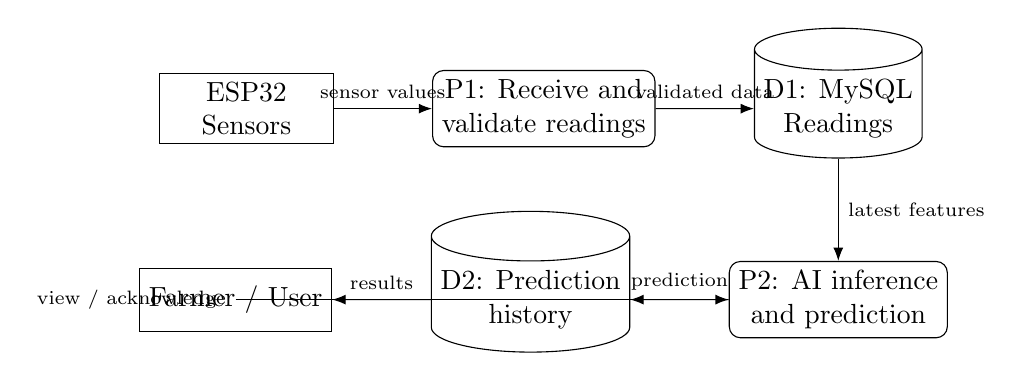
\begin{tikzpicture}[node distance=1.3cm and 1.25cm, >=Latex,
entity/.style={draw, rectangle, minimum width=2.2cm, minimum height=0.8cm, align=center},
process/.style={draw, rounded corners, minimum width=2.7cm, minimum height=0.9cm, align=center},
store/.style={draw, cylinder, shape border rotate=90, aspect=0.25, minimum width=1.8cm, minimum height=0.9cm, align=center}]
\node[entity] (esp) {ESP32\\Sensors};
\node[process, right=of esp] (ingest) {P1: Receive and\\validate readings};
\node[store, right=of ingest] (db) {D1: MySQL\\Readings};
\node[process, below=of db] (ai) {P2: AI inference\\and prediction};
\node[store, left=of ai] (pred) {D2: Prediction\\history};
\node[entity, left=of pred] (farmer) {Farmer / User};
\draw[->] (esp) -- node[above,align=center,font=\scriptsize]{sensor values} (ingest);
\draw[->] (ingest) -- node[above,font=\scriptsize]{validated data} (db);
\draw[->] (db) -- node[right,font=\scriptsize]{latest features} (ai);
\draw[->] (ai) -- node[above,font=\scriptsize]{prediction} (pred);
\draw[->] (pred) -- node[above,font=\scriptsize]{results} (farmer);
\draw[->] (farmer) |- node[left,font=\scriptsize]{view / acknowledge} (ai);
\end{tikzpicture}
\caption{Level 1 DFD for sensor ingestion, prediction, storage, and user review.}
\end{figure}

\section{Use Case Diagram}
\begin{figure}[H]
\centering
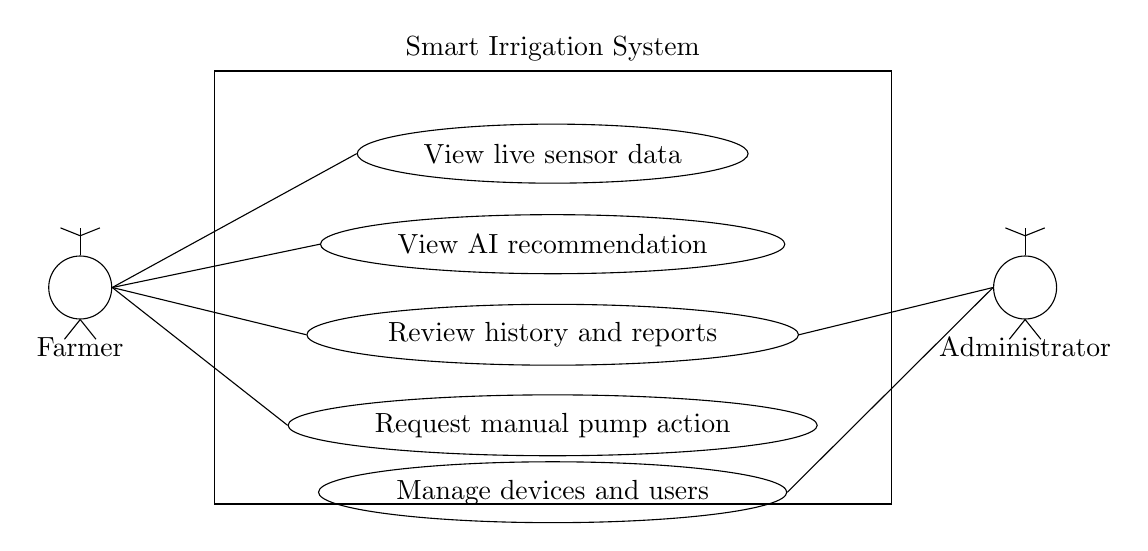
\begin{tikzpicture}[>=Latex, actor/.style={draw, circle, minimum size=0.8cm}, usecase/.style={draw, ellipse, minimum width=2.6cm, minimum height=0.75cm, align=center}, boundary/.style={draw, rectangle, minimum width=8.6cm, minimum height=5.5cm}]
\node[actor] (farmer) at (0,0) {};
\node[below=0.1cm of farmer] {Farmer};
\draw (farmer.north) -- ++(0,0.35);
\draw (farmer.north) ++(0,0.25) -- ++(-0.25,0.1);
\draw (farmer.north) ++(0,0.25) -- ++(0.25,0.1);
\draw (farmer.south) -- ++(-0.2,-0.25);
\draw (farmer.south) -- ++(0.2,-0.25);
\node[actor] (admin) at (12,0) {};
\node[below=0.1cm of admin] {Administrator};
\draw (admin.north) -- ++(0,0.35);
\draw (admin.north) ++(0,0.25) -- ++(-0.25,0.1);
\draw (admin.north) ++(0,0.25) -- ++(0.25,0.1);
\draw (admin.south) -- ++(-0.2,-0.25);
\draw (admin.south) -- ++(0.2,-0.25);
\node[boundary] (sys) at (6,0) {};
\node[above] at (6,2.75) {Smart Irrigation System};
\node[usecase] (view) at (6,1.7) {View live sensor data};
\node[usecase] (pred) at (6,0.55) {View AI recommendation};
\node[usecase] (hist) at (6,-0.6) {Review history and reports};
\node[usecase] (pump) at (6,-1.75) {Request manual pump action};
\node[usecase] (manage) at (6,-2.6) {Manage devices and users};
\draw (farmer.east) -- (view.west);
\draw (farmer.east) -- (pred.west);
\draw (farmer.east) -- (hist.west);
\draw (farmer.east) -- (pump.west);
\draw (admin.west) -- (manage.east);
\draw (admin.west) -- (hist.east);
\end{tikzpicture}
\caption{Use case diagram showing farmer and administrator interactions.}
\end{figure}

\section{Activity Diagram}
\begin{figure}[H]
\centering
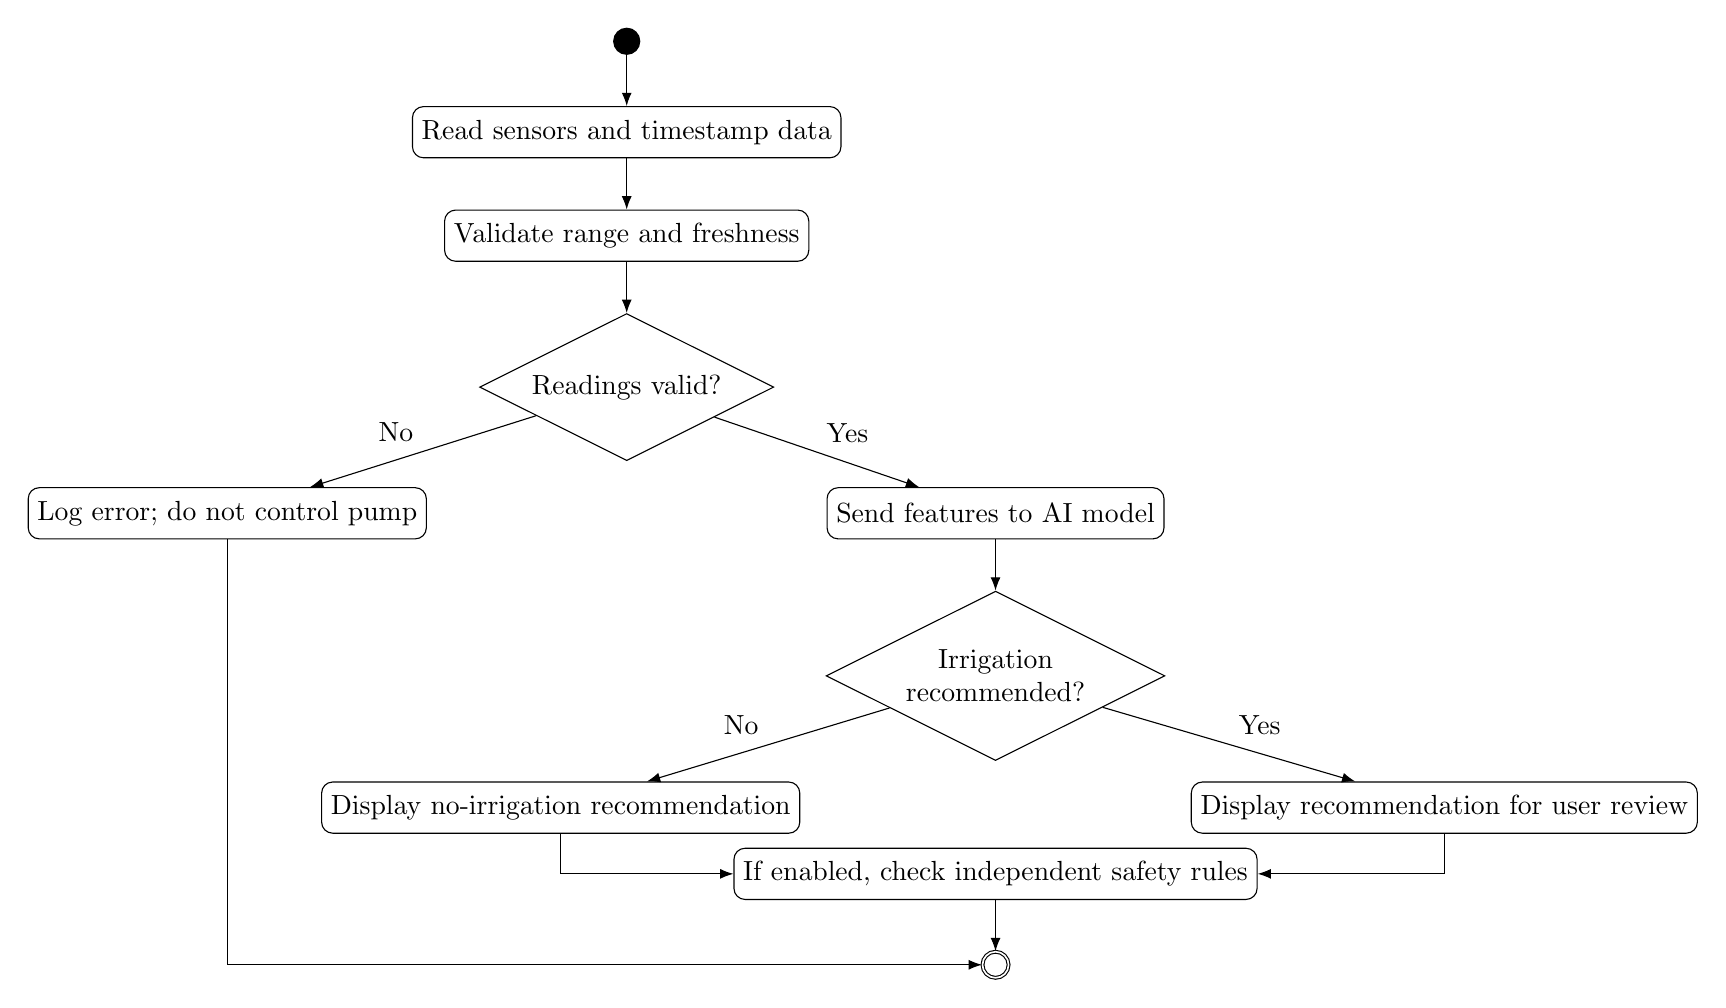
\begin{tikzpicture}[node distance=0.65cm, >=Latex,
start/.style={circle,draw,fill=black,minimum size=0.22cm},
end/.style={circle,draw,minimum size=0.32cm,double},
action/.style={draw,rounded corners,minimum width=4.2cm,minimum height=0.65cm,align=center},
decision/.style={draw,diamond,aspect=2,minimum width=2.6cm,align=center}]
\node[start] (s) {};
\node[action,below=of s] (read) {Read sensors and timestamp data};
\node[action,below=of read] (valid) {Validate range and freshness};
\node[decision,below=of valid] (ok) {Readings valid?};
\node[action,below left=0.8cm and 1.6cm of ok] (error) {Log error; do not control pump};
\node[action,below right=0.8cm and 1.6cm of ok] (infer) {Send features to AI model};
\node[decision,below=of infer] (need) {Irrigation\\recommended?};
\node[action,below left=0.8cm and 1.4cm of need] (no) {Display no-irrigation recommendation};
\node[action,below right=0.8cm and 1.4cm of need] (yes) {Display recommendation for user review};
\node[action,below=1.1cm of need] (safe) {If enabled, check independent safety rules};
\node[end,below=of safe] (e) {};
\draw[->] (s) -- (read);
\draw[->] (read) -- (valid);
\draw[->] (valid) -- (ok);
\draw[->] (ok) -- node[above left]{No} (error);
\draw[->] (ok) -- node[above right]{Yes} (infer);
\draw[->] (infer) -- (need);
\draw[->] (need) -- node[above left]{No} (no);
\draw[->] (need) -- node[above right]{Yes} (yes);
\draw[->] (no) |- (safe);
\draw[->] (yes) |- (safe);
\draw[->] (error) |- (e);
\draw[->] (safe) -- (e);
\end{tikzpicture}
\caption{Activity diagram for a safe recommendation workflow.}
\end{figure}

\section{Entity Relationship Diagram}
\begin{figure}[H]
\centering
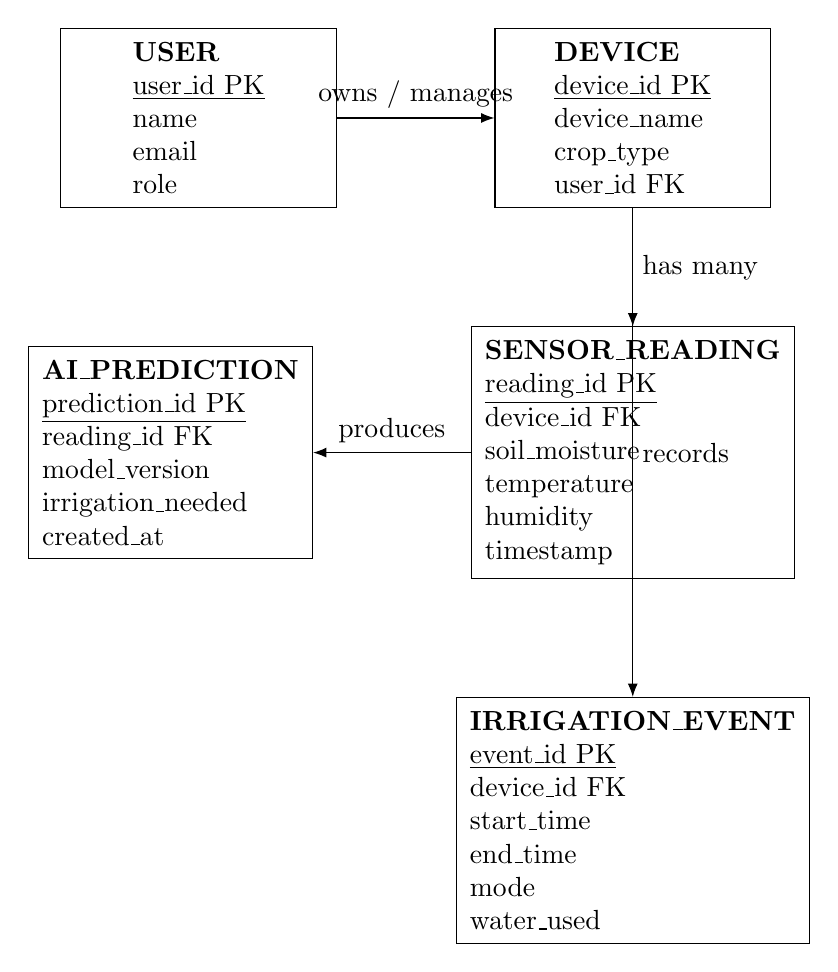
\begin{tikzpicture}[>=Latex, entity/.style={draw,rectangle,align=left,minimum width=3.5cm,inner sep=5pt}]
\node[entity] (user) {\textbf{USER}\\\underline{user\_id PK}\\name\\email\\role};
\node[entity, right=2.0cm of user] (device) {\textbf{DEVICE}\\\underline{device\_id PK}\\device\_name\\crop\_type\\user\_id FK};
\node[entity, below=1.5cm of device] (reading) {\textbf{SENSOR\_READING}\\\underline{reading\_id PK}\\device\_id FK\\soil\_moisture\\temperature\\humidity\\timestamp};
\node[entity, left=2.0cm of reading] (prediction) {\textbf{AI\_PREDICTION}\\\underline{prediction\_id PK}\\reading\_id FK\\model\_version\\irrigation\_needed\\created\_at};
\node[entity, below=1.5cm of reading] (event) {\textbf{IRRIGATION\_EVENT}\\\underline{event\_id PK}\\device\_id FK\\start\_time\\end\_time\\mode\\water\_used};
\draw[->] (user) -- node[above]{owns / manages} (device);
\draw[->] (device) -- node[right]{has many} (reading);
\draw[->] (reading) -- node[above]{produces} (prediction);
\draw[->] (device) -- node[right]{records} (event);
\end{tikzpicture}
\caption{ERD with primary keys (PK) and foreign keys (FK).}
\end{figure}

\section{Class Diagram}
\begin{figure}[H]
\centering
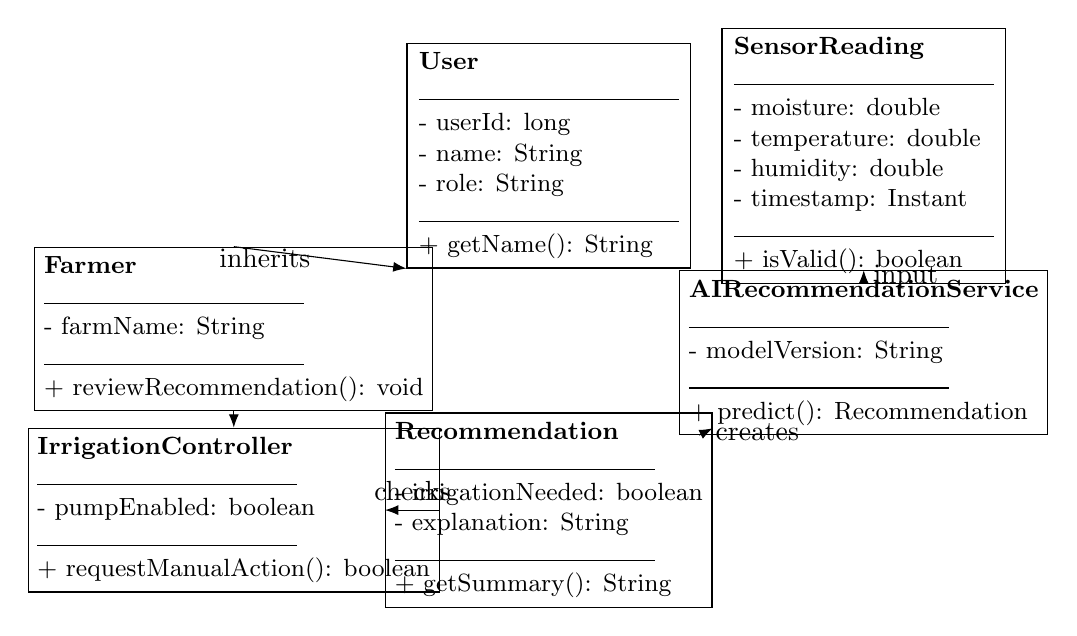
\begin{tikzpicture}[class/.style={draw,rectangle,align=left,minimum width=3.6cm,font=\small}, >=Latex]
\node[class] (user) at (0,0) {\textbf{User}\\\rule{3.3cm}{0.4pt}\\- userId: long\\- name: String\\- role: String\\\rule{3.3cm}{0.4pt}\\+ getName(): String};
\node[class] (farmer) at (-4,-2.2) {\textbf{Farmer}\\\rule{3.3cm}{0.4pt}\\- farmName: String\\\rule{3.3cm}{0.4pt}\\+ reviewRecommendation(): void};
\node[class] (reading) at (4,0) {\textbf{SensorReading}\\\rule{3.3cm}{0.4pt}\\- moisture: double\\- temperature: double\\- humidity: double\\- timestamp: Instant\\\rule{3.3cm}{0.4pt}\\+ isValid(): boolean};
\node[class] (service) at (4,-2.5) {\textbf{AIRecommendationService}\\\rule{3.3cm}{0.4pt}\\- modelVersion: String\\\rule{3.3cm}{0.4pt}\\+ predict(): Recommendation};
\node[class] (recommend) at (0,-4.5) {\textbf{Recommendation}\\\rule{3.3cm}{0.4pt}\\- irrigationNeeded: boolean\\- explanation: String\\\rule{3.3cm}{0.4pt}\\+ getSummary(): String};
\node[class] (controller) at (-4,-4.5) {\textbf{IrrigationController}\\\rule{3.3cm}{0.4pt}\\- pumpEnabled: boolean\\\rule{3.3cm}{0.4pt}\\+ requestManualAction(): boolean};
\draw[->] (farmer.north) -- node[left]{inherits} (user.south west);
\draw[->] (service) -- node[right]{creates} (recommend);
\draw[->] (reading) -- node[right]{input} (service);
\draw[->] (controller) -- node[above]{checks} (recommend);
\draw[->] (farmer) -- (controller);
\end{tikzpicture}
\caption{Core class diagram; implementation may add repository and device-communication classes.}
\end{figure}

\section{Object Diagram}
\begin{figure}[H]
\centering
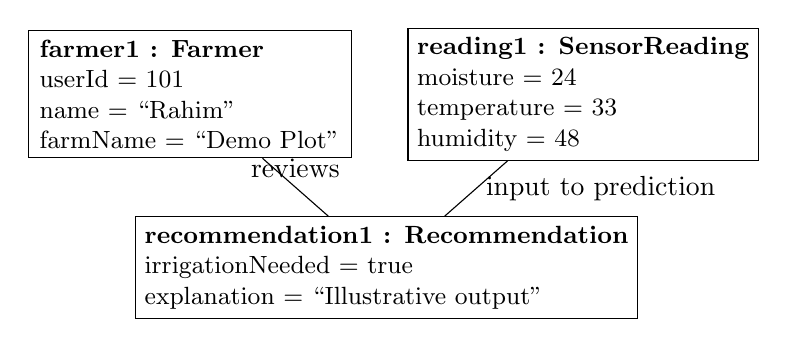
\begin{tikzpicture}[obj/.style={draw,rectangle,align=left,minimum width=4.1cm,font=\small}]
\node[obj] (f) at (0,0) {\textbf{farmer1 : Farmer}\\userId = 101\\name = ``Rahim''\\farmName = ``Demo Plot''};
\node[obj] (r) at (5,0) {\textbf{reading1 : SensorReading}\\moisture = 24\\temperature = 33\\humidity = 48};
\node[obj] (p) at (2.5,-2.2) {\textbf{recommendation1 : Recommendation}\\irrigationNeeded = true\\explanation = ``Illustrative output''};
\draw[-] (f) -- node[above]{reviews} (p);
\draw[-] (r) -- node[right]{input to prediction} (p);
\end{tikzpicture}
\caption{Illustrative object instances at one moment in time. Values are examples, not validated field data.}
\end{figure}

\chapter{Implementation Plan and Interface Prototype}
\section{Suggested Software Structure}
\begin{itemize}[leftmargin=*]
\item \textbf{Device layer:} ESP32 firmware reads sensors and publishes MQTT messages.
\item \textbf{Backend layer:} Java Spring Boot validates readings, exposes REST endpoints, and coordinates inference.
\item \textbf{Data layer:} MySQL stores devices, readings, predictions, and irrigation events.
\item \textbf{AI layer:} a trained Decision Tree or Random Forest is served through a Python API or a compatible Java inference runtime.
\item \textbf{UI layer:} a browser dashboard shows readings, recommendations, and history.
\end{itemize}

\section{Java Class Responsibilities}
The initial class design includes at least five classes: \texttt{User}, \texttt{Farmer}, \texttt{SensorReading}, \texttt{Recommendation}, \texttt{AIRecommendationService}, and \texttt{IrrigationController}. The supplied desktop prototype uses these classes to demonstrate object-oriented structure. It is a user-interface prototype, not a complete cloud-connected application.

\section{Prototype Features}
\begin{itemize}[leftmargin=*]
\item Input soil moisture, temperature, and humidity values.
\item Validate that values are within configured demo ranges.
\item Generate an explicitly labeled demonstration recommendation.
\item Display a recommendation summary in the interface.
\item Keep pump action disabled in the supplied prototype.
\end{itemize}

\section{Important AI Implementation Note}
The included desktop interface uses a clearly marked demonstration recommendation service so the interface can run before a trained model is available. Its output must not be described as a trained AI prediction. Replace the demonstration implementation with an evaluated model integration before claiming live AI functionality.

\chapter{Testing and Evaluation}
\section{Test Plan}
\begin{longtable}{p{0.12\textwidth}p{0.34\textwidth}p{0.42\textwidth}}
\toprule
\textbf{Test ID} & \textbf{Test} & \textbf{Expected result}\\
\midrule
T-01 & Enter valid sensor values & Values accepted and displayed.\\
T-02 & Enter moisture outside configured range & Input rejected with a clear message.\\
T-03 & Submit a prediction request & A demo recommendation is displayed; later, the trained model response is displayed.\\
T-04 & Send missing sensor fields & Backend rejects or marks the record invalid.\\
T-05 & Simulate a stale reading & No pump command is issued.\\
T-06 & Simulate MQTT/network failure & UI reports device offline; no indefinite pump operation.\\
T-07 & Evaluate the trained model on held-out data & Metrics and confusion matrix are saved in the report.\\
T-08 & Compare AI with baseline rule & Report both results using the same test protocol.\\
T-09 & Attempt pump command with safety condition failed & Command is blocked.\\
T-10 & Review historical data & Records are shown in chronological order.\\
\bottomrule
\end{longtable}

\section{AI Evaluation Metrics}
Report accuracy, precision, recall, F1-score, and the confusion matrix. Prioritize recall for the irrigation-needed class while also reporting false-positive recommendations, because unnecessary irrigation also has a cost. Use a final test set not used for model selection. Document the dataset, label-generation method, and known limitations.

\chapter{Expected Outcomes}
\begin{enumerate}[leftmargin=*]
\item A documented project proposal and requirements specification.
\item Six system diagrams.
\item A working sensor-data capture prototype.
\item A Java application prototype with a class-based interface.
\item A database design for readings and predictions.
\item An evaluated machine-learning model or a clearly documented model-training pipeline.
\item Test results, risk analysis, and final presentation.
\end{enumerate}

\chapter{Future Enhancements}
Potential future work includes crop-specific model evaluation, rainfall forecast integration, water-flow measurement, abnormal sensor detection, mobile notifications, multiple field support, and safe automated irrigation after field validation.

\chapter{Conclusion}
The proposed system combines IoT sensing, machine learning, and Java software engineering to support irrigation decisions. The initial version focuses on sensor monitoring, reliable data storage, and transparent recommendations. Its success will be assessed through functional tests and an honest evaluation of the AI model against a documented baseline. Automatic pump control will remain protected by independent safety limits and will not rely on an unvalidated model alone.

\chapter{References}
\begin{enumerate}[leftmargin=*]
\item Scikit-learn documentation, \url{https://scikit-learn.org/stable/}.
\item Spring Boot documentation, \url{https://spring.io/projects/spring-boot}.
\item Eclipse Paho MQTT client documentation, \url{https://eclipse.dev/paho/}.
\item MySQL documentation, \url{https://dev.mysql.com/doc/}.
\item FAO AQUASTAT, \url{https://www.fao.org/aquastat/en/}.
\item UCI Machine Learning Repository, \url{https://archive.ics.uci.edu/}.
\end{enumerate}

\appendix
\chapter{Submission Notes}
Replace the student details on the cover page. Confirm that the course instructor accepts a Java desktop prototype for the interface requirement. If the instructor requires a web interface, implement the same classes behind a Spring Boot web application and use HTML/CSS/JavaScript for the browser UI. Add actual implementation screenshots, dataset provenance, measured model results, and the final test evidence before submission.
\end{document}
